%auto-ignore
\providecommand{\MainFolder}{..}
\documentclass[\MainFolder/Text.tex]{subfiles}
\begin{document}

\section{String topology and Chen's iterated integrals}

String topology of a manifold~$M$ is the study of the \emph{free loop space} $\Loop M = \{\gamma: \Sph{1}\rightarrow M\text{ continuous}\}$ and natural structures on it. Each loop~$\gamma$ is parametrized, with base-point~$\gamma(1)$, and there is a natural $\Sph{1}$-action changing the base-point. This gives rise to two homology theories:
\begin{center}
\begin{tabular}{rl}
 $\H(\Loop M)\quad\dotsc$& the \emph{singular homology} and \\[1ex]
 $\H^{\Sph{1}}\!(\Loop M)\quad\dotsc$ & \parbox[t]{10cm}{the \emph{equivariant homology} --- ``the singular homology of the space of parametrized loops with the base-point forgotten.''}
\end{tabular}
\end{center}
In this thesis, we restrict to $\H^{\Sph{1}}\!(\Loop M)$ only. We also use $\R$-coefficients implicitly, although the topological constructions work with any coefficients.

If $M$ is an oriented surface, there is a bracket $\StringOp_2$ and a cobracket $\StringCoOp_2$ on the equivariant homology, which can be described as follows (we assume the counterclockwise orientation and transversality of the intersection):
%\footnote{If one wishes, and is allowed to, one can cut holes inside of the loops and make some non-contractible.}
\begin{equation}\label{Eq:ConstrLoop}
\begin{aligned}
\StringOp_2\left(
\parbox[c]{2.85cm}{
\begin{tikzpicture}
	\def\rad{.8cm}
	\draw[green,thick,decoration={markings, mark=at position 0.25 with {\arrow{>}}},postaction={decorate}] ([shift=(0:\rad)]0,0) arc (0:360:\rad);  
	%\draw[green,thick,dotted] ([shift=(280:\rad)]0,0) arc (280:360:\rad);
	\draw[red,thick,decoration={markings, mark=at position 0.25 with {\arrow{>}}},postaction={decorate}] (1.5*\rad,0) circle (\rad);
	\end{tikzpicture}}
\right)
&=\parbox[c]{2.85cm}{
\begin{tikzpicture}
	\def\rad{.8cm}
	\draw[blue,thick] ([shift=(90:\rad)]0,0) arc (90:360:\rad); %Big loop on the lft
    \draw[blue,thick] ([shift=(0:\rad)]0,0) arc (0:180:.25*\rad); %Small connecting loop
	\draw[blue,thick] ([shift=(180:\rad)]1.5*\rad,0) arc (180:450:\rad); %Big loop on the right
	\draw[blue,thick,decoration={markings, mark=at position 0.5 with {\arrow{<}}},
        postaction={decorate}] ([shift=(90:\rad)]0,0) to ([shift=(90:\rad)]1.5*\rad,0); %The oriented connecting line
\end{tikzpicture}}
\ -\ 
\parbox[c]{2.85cm}{
\begin{tikzpicture}
	\def\rad{.8cm}
	\draw[blue,thick] ([shift=(0:\rad)]0,0) arc (0:270:\rad); %Big loop on the left
	\draw[blue,thick] ([shift=(180:\rad)]1.5*\rad,0) arc (180:360:.25*\rad); %Small connecting loop
	\draw[blue,thick] ([shift=(270:\rad)]1.5*\rad,0) arc (270:540:\rad); %Big loop on the right
	\draw[blue,thick,decoration={markings, mark=at position 0.5 with {\arrow{>}}},
        postaction={decorate}] ([shift=(270:\rad)]0,0) to ([shift=(270:\rad)]1.5*\rad,0);
\end{tikzpicture}}\quad\text{and}\\
\StringCoOp_2\left(\hspace{-.4em}
\parbox[c]{3.3cm}{
\begin{tikzpicture}
	\def\rad{.8cm}
	\draw[blue,thick,decoration={markings, mark=at position 0.25 with {\arrow{>}}},
        postaction={decorate}] ([shift=(45:\rad)]0,0) arc (45:315:\rad);
	\draw[blue,thick,decoration={markings, mark=at position 0.25 with {\arrow{<}}},
        postaction={decorate}] ([shift=(-135:\rad)]2*\rad,0) arc (-135:135:\rad);
	\draw[blue,thick] (45:\rad) to[out=-45,in=135] ($(-135:\rad)+(2*\rad,0)$);
	\draw[blue,thick] (-45:\rad) to[out=45,in=225] ($(135:\rad)+(2*\rad,0)$);
\end{tikzpicture}}\right)
&=\parbox[c]{1.64cm}{
\begin{tikzpicture}
\def\rad{.8cm}
\draw[green,thick,decoration={markings, mark=at position 0.25 with {\arrow{>}}},
        postaction={decorate}] (0,0) circle (\rad);
\end{tikzpicture}}\otimes
\parbox[c]{1.64cm}{
\begin{tikzpicture}
\def\rad{.8cm}
\draw[red,thick,decoration={markings, mark=at position 0.25 with {\arrow{<}}},
        postaction={decorate}] (0,0) circle (\rad);
\end{tikzpicture}}\ -\ 
\parbox[c]{1.64cm}{
\begin{tikzpicture}
\def\rad{.8cm}
\draw[red,thick,decoration={markings, mark=at position 0.25 with {\arrow{<}}},
        postaction={decorate}] (0,0) circle (\rad);
\end{tikzpicture}} \otimes
\parbox[c]{1.64cm}{
\begin{tikzpicture}
\def\rad{.8cm}
\draw[green,thick,decoration={markings, mark=at position 0.25 with {\arrow{>}}},
        postaction={decorate}] (0,0) circle (\rad);
\end{tikzpicture}}
\end{aligned}
\end{equation}
\begin{description}[leftmargin=*]
 \item[$\StringOp_2$:] Put one base-point on the first loop and another base-point on the second loop in all possible positions. Whenever the two base-points overlap, connect the two loops by running first along the first loop and next along the second loop, starting and ending at the overlap. Forget the base-point of the newly obtained loop and multiply it with the sign of the intersection. Should more overlaps occur, take the sum.
 \item[$\StringCoOp_2$:] Put two ordered base-points on the same loop in all possible positions. Whenever they overlap with a non-zero phase, disconnect the loop into two and form a tensor product as follows. The first loop in the tensor product is the portion of the original loop running from the first base-point to the second. The second loop is  the portion running from the second base-point to the first. Forget the base-point and multiply it with the sign of the intersection. Should more overlaps occur, take the sum of the resulting tensors.
\end{description}
These operations are known as the \emph{Goldman bracket} and the \emph{Turaev cobracket} and were defined and studied in \cite{Goldman1986} and \cite{Turaev1991}, respectively.

In \cite{Sullivan1999}, it was demonstrated that~$\StringOp_2$ generalizes to families of loops and to an arbitrary dimension~$n$ of an oriented manifold~$M$. The coproduct $\StringCoOp_2$ also generalizes, which is explained in \cite{Basu2011}. The picture is precisely~\eqref{Eq:ConstrLoop}, just the intersection points come from transverse intersections of smooth $k$-chains in $M$. In order to make this construction rigorous, the most straightforward way is to use a geometric homology theory based on smooth chains, so that the transverse intersection of two smooth chains is again a smooth chain. Such theory for smooth manifolds was constructed in \cite{Lipyanskiy2014}.

The main theorem of \cite{Chas2004} asserts that $\StringOp_2$ and $\StringCoOp_2$ induce the structure of an \emph{involutive bi-Lie algebra} (abbreviated $\IBL$-algebra) of degree $(2-n)$ on the reduced equivariant homology $\bar{\H}^{\Sph{1}}\!(\Loop M) = H^{\Sph{1}}\!(\Loop M,M)$, i.e., the homology relative to constant loops $M\xhookrightarrow{}\Loop M$. The reduced homology is necessary for $\StringCoOp_2$ to be well-defined because of the phenomenon of ``vanishing of small loops'':  Let $\sigma\in C_1(\Loop M)$ be a $1$-chain which on its one end agrees with the loop in the argument of $\StringCoOp_2$ in \eqref{Eq:ConstrLoop}, and as it continues to the other end, the left knot contracts to the mid-point until just the right knot is left. It is then easy to see that $ 0 \neq \Bdd \StringCoOp_2(\sigma) - \StringCoOp_2(\Bdd \sigma) \in C(M)\otimes C(\Loop M) + C(\Loop M)\otimes C(M)$. In fact, there might also be a problem with the restriction of $\StringOp_2$ to $\bar{\H}^{\Sph{1}}\!(\Loop M)$ since the constant loops might not form an ideal (e.g., the case of $\T^2$). Our current understanding of this issue is that there should be an $\IBL$-structure either on $\H^{\Sph{1}}\!(\Loop M)$ when the Euler characteristics $\chi(M)$ vanishes, or on the point-reduced version $\H^{\Sph{1}}\!(\Loop M,\mathrm{pt})$ when $\chi(M) \neq 0$. However, the extension of $\StringCoOp_2$ requires choices (of a nowhere vanishing vector field), and it is not clear to which extent they influence the $\IBL$-structure. These problems are addressed in the work in progress \cite{Cieliebak2018}, where Poincar\'e duality on the symplectic homology of the unit cotangent bundle is introduced and related to the (non-equivariant) string topology. We continue to use $\bar{\H}^{\Sph{1}}\!(\Loop M)$ as an avatar for either $\H^{\Sph{1}}\!(\Loop M)$ or $\H^{\Sph{1}}\!(\Loop M,\mathrm{pt})$.

It is expected that the $\IBL$-structure on $\bar{\H}^{\Sph{1}}\!(\Loop M)$ is induced from a much richer algebraic structure on the chain level. In fact, there is the algebraic notion of a strong homotopy involutive bi-Lie algebra (abbreviated $\IBLInfty$-algebra) which was developed in \cite{Cieliebak2015}. It consists of operations $(\OPQ_{klg})$ for $k$, $l \ge 1$, $g\ge 0$, where $\OPQ_{110}$ is a boundary operator, $\OPQ_{210}$ a bracket and $\OPQ_{120}$ a cobracket, which satisfy the $\IBL$-relations up to higher homotopies $(\OPQ_{klg})$. Consider the string space $\StringSpace M = (\EG\Sph{1}\times \Loop M)/\Sph{1}$ (the homotopically correct version of the quotient $\Loop M/\Sph{1}$), and let $(C(\StringSpace M),\Bdd)$ be the geometric chain complex of $\StringSpace M$ where~$\StringOp_2$ and $\StringCoOp_2$ are partially defined on transverse smooth chains. An \emph{$\IBLInfty$-chain model for equivariant string topology} is an $\IBLInfty$-algebra $(\Model(\StringSpace M),(\OPQ_{klg}))$ together with an $\IBLInfty$-morphism
$$ (C(\StringSpace M),\Bdd,\StringOp_2,\StringCoOp_2) \xrightarrow{(\HTP_{klg})} (\Model(\StringSpace M),\OPQ_{110},\OPQ_{210},\OPQ_{120},(\OPQ_{klg})) $$
which induces an isomorphism of the reduced homologies with respect to $\Bdd$ and $\OPQ_{110}$ (we assume that $\Model(\StringSpace M)$ has a proper reduced version).

As a properad, $\IBLInfty$ is a quasi-free resolution of the properad $\IBL$ and thus has convenient homotopy theoretical properties; e.g., homotopy inverses of quasi-isomorphisms exist. They imply that any two weakly homotopy equivalent (zig-zag of quasi-isomorphisms) $\IBLInfty$-algebras are (strongly) homotopy equivalent, and hence an $\IBLInfty$-chain model of the equivariant string topology is unique up to an $\IBLInfty$-homotopy.


In this thesis, we use perturbative Chern-Simons theory to construct an $\IBLInfty$-chain model for the equivariant string topology of an oriented compact Riemannian manifold~$M$ based on the space of cyclic Hochschild cochains of the de Rham cohomology $\HDR\coloneqq \HDR(M)$. It is the original idea of \cite{Cieliebak2015}, and the proofs that this construction works are under development in \cite{Cieliebak2018} and \cite{Cieliebak2018b}. We explain the $\IBLInfty$-chain model with a physical flavor. 

Let $\BCyc \DR$, where $\DR \coloneqq \DR(M)$ be the graded vector space generated by cyclic words 
$$ \omega_1\dotsb\omega_k = (-1)^{\Abs{\omega_k}(\Abs{\omega_1}+\dotsb+\Abs{\omega_k})} \omega_k\omega_1 \dotsb \omega_{k-1} $$
for homogenous $\omega_1$, $\dotsc$, $\omega_k \in \DR$ with $k\ge 1$ (reduced cyclic bar complex). The grading satisfies $\Abs{\omega_i} = \Deg(\omega_i) - 1$, where $\Deg(\omega_i)$ denotes the form-degree of $\omega_i$. On $\BCyc \DR$, we consider the cyclic Hochschild differential
$$ \Hd(\omega_1 \dotsb \omega_k) = \begin{aligned}[t]
&\sum_{i=1}^k (-1)^{\Abs{\omega_1} + \dotsb + \Abs{\omega_{i-1}}}\omega_1 \dotsb\Dd\omega_i\dotsb \omega_k \\
+&\sum_{i=1}^{k-1} (-1)^{\Abs{\omega_1}+\dotsb + \Abs{\omega_{i-1}} + \Abs{\omega_i} + 1}\omega_1 \dotsb \omega_i \wedge \omega_{i+1} \dotsb \omega_k\\
+&(-1)^{\Abs{\omega_k}(\Abs{\omega_1} + \dotsb + \Abs{\omega_{k-1}}) + \Abs{\omega_k} + 1}\omega_k \wedge \omega_1 \dotsb \omega_{k-1}.
\end{aligned}$$
It descends from the Hochschild differential on the bar construction $\B \DR$, which is the sum of the unique extensions of degree shifts of $\Dd$ and $\wedge$ to coderivatives. The \emph{Chen's iterated integrals map} is the map
$$ I: \begin{aligned}[t]
    \BCyc \DR& \longrightarrow C^*(\StringSpace M)\\    
    \omega_1 \dotsb \omega_k & \longmapsto  \Bigl(\sigma \mapsto \varepsilon(\omega) \int_{K_\sigma \times \Delta^k} \omega_1(\tilde{\sigma}(x,t_1)) \dotsb \omega_k(\tilde{\sigma}(x,t_k))\Bigr),
   \end{aligned}$$
where $\varepsilon(\omega)$ is the sign
$$ \varepsilon(\omega) = (-1)^{(k-1)(\Abs{\omega_1} + 1) + (k-2)(\Abs{\omega_2} + 1) + \dotsb + \Abs{\omega_{k-1}} + 1}, $$
the map $\tilde{\sigma}: K_\sigma\times\Sph{1} \rightarrow M$ is the projection of a lift $K_\sigma \xrightarrow{\hspace{.2em}\sigma\hspace{.2em}}\StringSpace M \dasharrow \EG \Sph{1} \times \Loop M$ to the second factor, and we identify $\Sph{1} = \R/\Z$. It is a chain map (with respect to the cohomological grading of $\BCyc\DR$ by $\Abs{\omega_1 \dotsc \omega_k} = \Abs{\omega_1} + \dotsb + \Abs{\omega_k}$), and if $\pi_1(M) = 0$, then it induces an isomorphism of the reduced homologies $\bar{\H}(\BCyc \DR,\Hd)$ and $\bar{\H}^*(\StringSpace M,\delta)$. Here, $\bar{\H}(\BCyc \DR,\Hd) \coloneqq \H(\RedBCyc \DR,\Hd)$, where $\RedBCyc \DR \coloneqq \coker(\BCyc \R \xhookrightarrow{} \BCyc\DR)$ and $\bar{\H}^*(\StringSpace M) \coloneqq \H^*(\StringSpace M)/\R[u]$, where the polynomial ring $\R[u]$, $\Abs{u} = 2$ comes from the module structure induced by $\StringSpace M = (\EG \Sph{1} \times \Loop M)/\Sph{1} \rightarrow \EG/\Sph{1} = \CP^{\infty}$ (see \cite{Cieliebak2013}). The proof of this isomorphism is the subject of \cite{Cieliebak2018b} and is based on \cite{Getzler} after identifying $(\BCyc \DR,\Hd)$ with the correct totalization of the Connes' cyclic bicomplex of $\DR$ up to a weak equivalence.

\section{IBL-infinity chain model and Chern-Simons theory}

We consider the \emph{dual cyclic bar complex}
$$ \CDBCyc \DR = (\BCyc\DR)^{\GD}, $$
where $\GD$ stands for the graded dual, with the dual Hochschild differential~$\Hd^*$. The hat indicates that $\CDBCyc \DR$ is the weight-completion of the (cyclic) cobar construction $\mathcal{C}_{\mathrm{cyc}} \DR^*$, which takes care of the bubbling of degree-$1$ forms (if $\omega\in \DR^1$, then $\Abs{\omega} = 0$) and constants~$1$ ($\Abs{1} = -1$). The dual of the Chen's iterated integral map provides a chain map 
$$I^*: (C(\StringSpace M),\Bdd) \rightarrow (\CDBCyc\DR,\Hd^*).$$
In this setting, we introduce the following physical intuition. The following discussion might be imprecise.
%and reflects the author's wild imagination in the night before submitting the thesis. For more serious mathematics, please, see the rest 250+ pages.

We think of
\begin{itemize}
\item elements of $\DR$ as \emph{fields,}
\item elements of $\BCyc \DR$ as \emph{field strings} (not to confuse with string-fields) and
\item elements of the space
$$ \Fun(\BCyc \DR) \coloneqq \Sym(\DBCyc\DR)\COtimes \R((\hbar)), $$
where $\R((\hbar))$ is the ring of Laurent series in Planck's constant $\hbar$, $\Sym$ denotes the symmetric algebra and $\hat{\otimes}$ is the completed tensor product, as \emph{observables on field strings.}
\end{itemize}
If $\sigma$ a string in $M$, the observable $I^*(\sigma)$ ``localizes'' on field strings which approximate $\sigma$; for instance, it holds $I^*(\omega) = \int_{\sigma} \omega$, and so $I^*(\omega)$ ``localizes'' at fundamental forms of $\sigma$. We keep the following picture in mind:
\begin{center}
 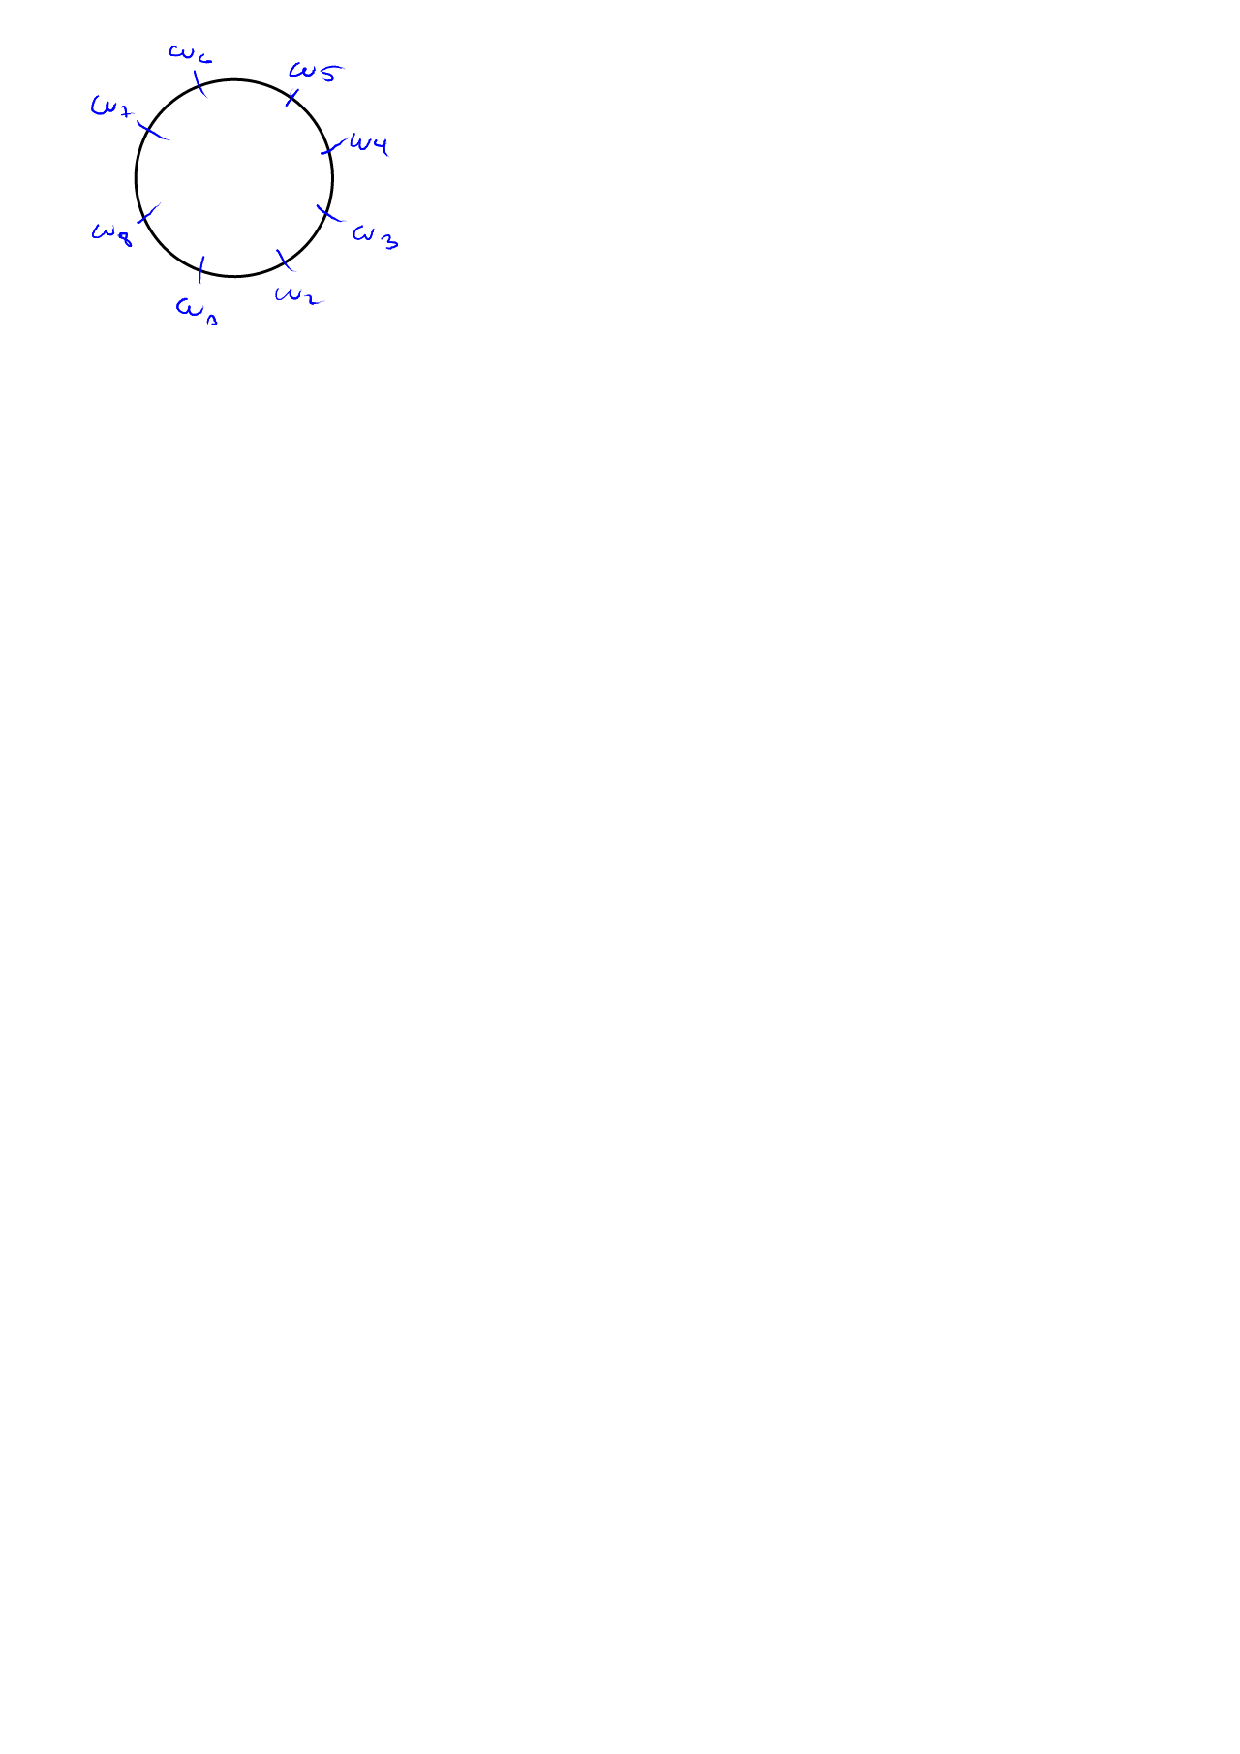
\includegraphics[trim=1.2cm 24cm 14cm .3cm]{\GraphicsFolder/kruh.pdf}
\end{center}
We are dealing with two ``dynamical'' theories. One is the theory of fields $\omega\in \DR(M)$ and one of field strings $\omega_1 \dotsb \omega_k \in \BCyc \DR$.

The field theory is at hand. We know that $(\DR,\Dd,\wedge,\langle\cdot,\cdot\rangle)$, where $\langle\omega_1,\omega_2\rangle = \int_M \omega_1 \wedge \omega_2$ for $\omega_1$, $\omega_2\in \DR$, is a \emph{symmetric dg-Frobenius algebra}. It is well-known that finite-dimensional Frobenius algebras $V$ are equivalent to $2$-dimensional topological quantum field theories, shortly TQFT. Finite-dimensionality is a sufficient (and necessary) condition so that the trivial cylinder, corresponding to the identity, satisfies $\Id = \sum \langle \cdot,e^i\rangle e_i$. For now, we will ignore this issue and work with $V = \DR$, although we will soon transfer to $\HDR$, where everything is just fine.
%One can also take the non-degenerate quotient of the small subalgebra of $\DR$ with respect to the canonical Hodge decomposition associated to a Riemannian metric on $M$. We denote it by $\VansQuotient(\VansSmall(\DR))$ and define in Chapter~\ref{Chap:5}. If our conjectures are correct, the results of our construction should be homotopy equivalent.
We will represent interactions of fields via Feynman graphs drawn on surfaces; i.e., the trivial cylinder for fields will be a line and the pair of pants $3$ segments emanating from one point.

Let us now consider field strings. The following diagram defines the operations $$ \OPQ_{210}: \hat{\Ext}_2 \DBCyc V \rightarrow \hat{\Ext}_1\DBCyc V \quad\text{and}\quad \OPQ_{120}: \hat{\Ext}_1\DBCyc V \rightarrow \hat{\Ext}_2\DBCyc V .$$
\begin{center}
 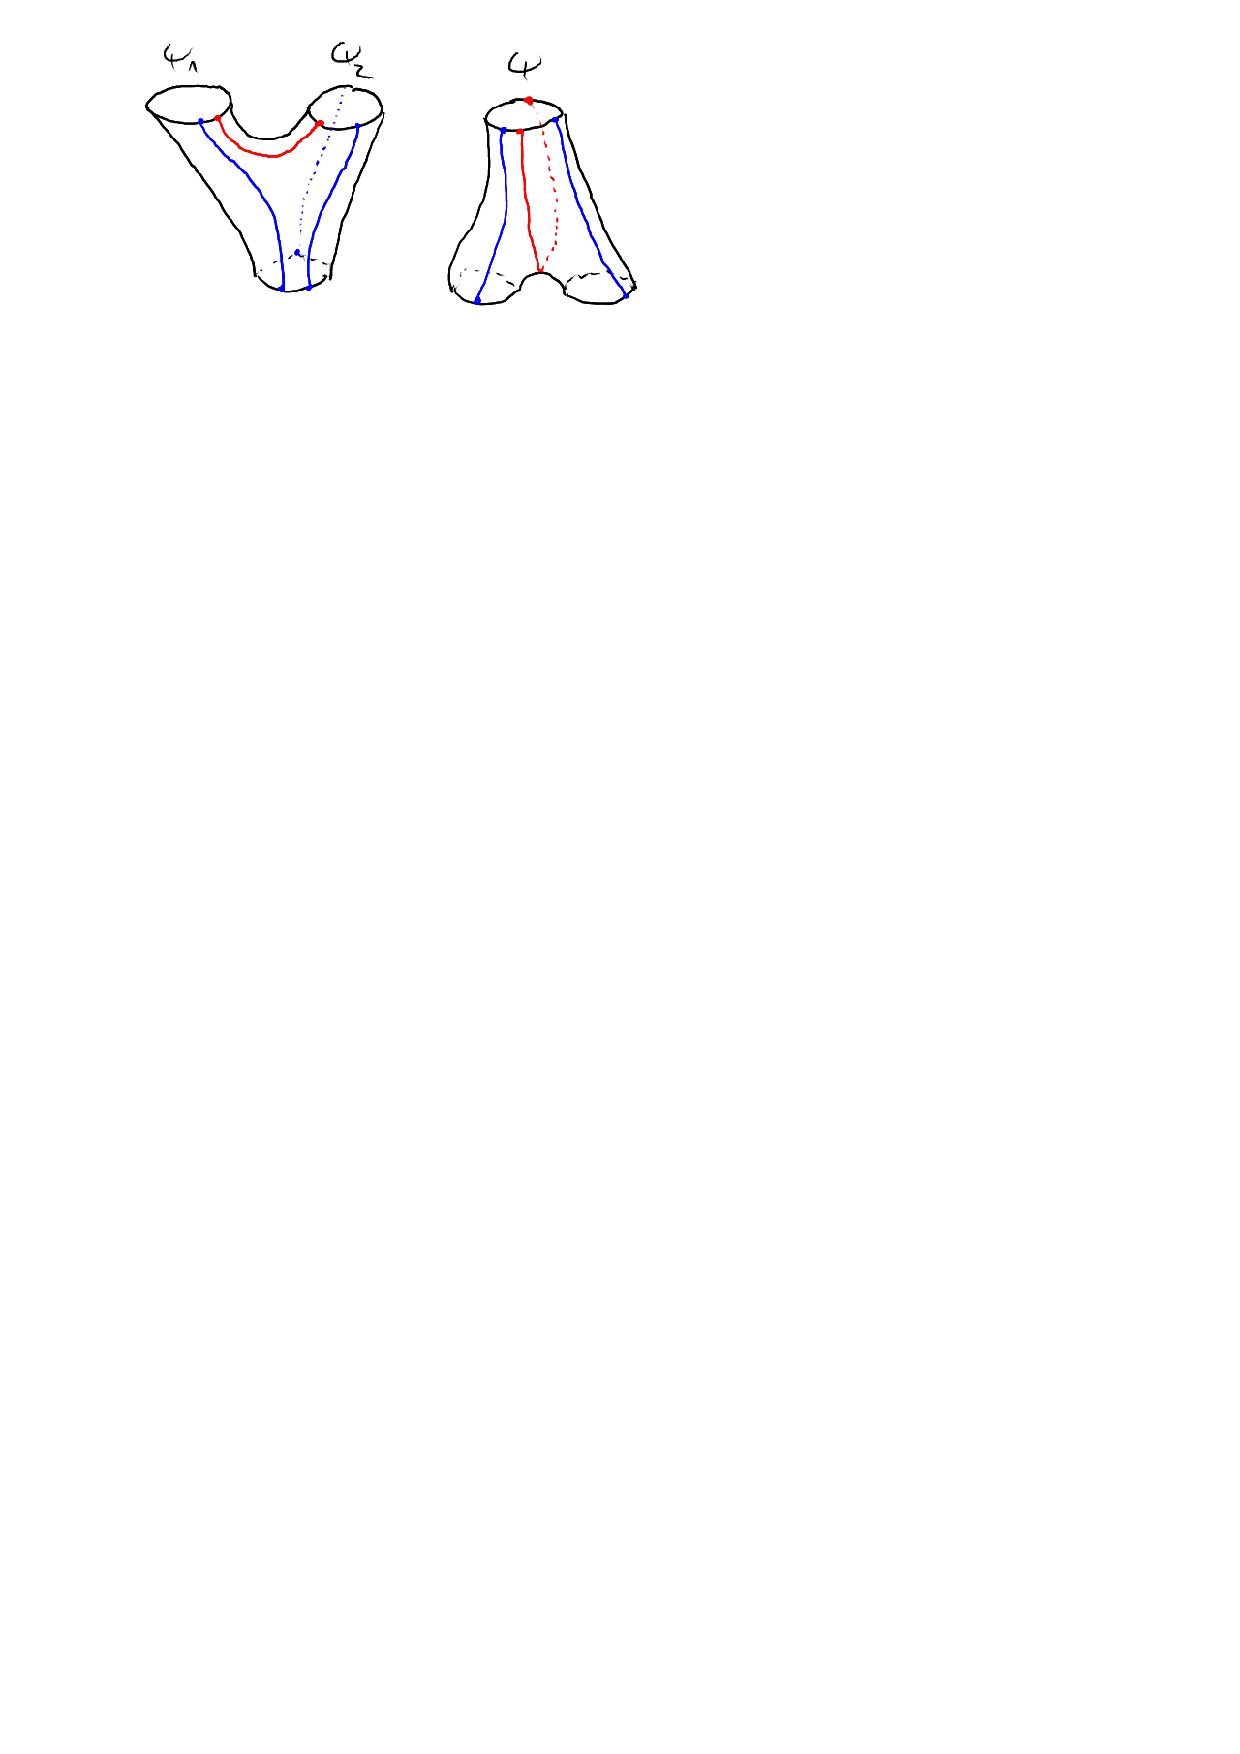
\includegraphics[trim=2cm 24cm 10cm .3cm]{\GraphicsFolder/op.pdf}
\end{center}
We read the diagram from the top to the bottom and imagine fields $\omega\in \DR$ propagating along the lines (one can also thing of $\omega$'s being fed into $\psi$'s from the bottom to the top).
%$I^*(\sigma)$ localizes which 
%The output string will be localized at any field string which arose by propagating the focalized string fields along the diagram. I.e. on those which are obtained by propagating those on which the input strings are non-zero along the diagram.
%
%From the point of view of the TQFT, these propagators are trivial cylinders, and hence nothing is happening. 
The picture suggests that $\OPQ_{210}$ and $\OPQ_{120}$ compute $\StringOp_2$ and $\StringCoOp_2$, respectively. The operations $\OPQ_{210}$ and $\OPQ_{120}$ were defined in \cite{Cieliebak2015} and make up an $\IBL$-algebra on $\DBCyc V$. We show that $\OPQ_{210}$ is obtained via cyclization of the Gerstenhaber bracket on Hochschild cochains and $\OPQ_{120}$ can be seen as a factorization with respect to the cyclic shuffle product of an extension of the Schwarz's $\BV$-operator on functions on $\DR$ to cyclic invariants. We construct a new $\BV$-operator
$$ \BVOp_{\mathrm{s}} \coloneqq  \hat{\OPQ}_{120} + \hbar \hat{\OPQ}_{210} $$
on $\Fun(\BCyc V)$, where the hats denote canonical extensions to derivatives of orders $1$ and $2$, respectively. We call $\BVOp_{\mathrm{s}}$ the \emph{string $\BV$-operator.} In physics, a $\BV$-operator $\BVOp$ on $\Fun(V)$ is related to the measure in the path integral $\int \mu$ over the space of fields. An action $S\in \Fun(V)$ satisfying the \emph{quantum master equation}
$$ \BVOp S + \frac{1}{2}\{S,S\} = 0 $$
defines a new measure $\int e^{-S} \mu$, and the corresponding twisted $\BV$-operator (or rather $\BVInfty$-operator) reads $\BVOp^S = e^{-S} \BVOp e^{S}$. On field strings, we define the following actions $S_{\mathrm{free}}$, $S_{\mathrm{int}}\in \Fun(\BCyc V)$, which remind us of the Chern-Simons functional:
$$S_{\mathrm{free}}(\omega_1 \omega_2) \coloneqq \pm \hbar^{-1}\int_M \omega_1 \wedge \Dd \omega_2 \quad\text{and}\quad S_{\mathrm{int}}(\omega_1 \omega_2 \omega_3) \coloneqq \pm \hbar^{-1}\int_M \omega_1 \wedge \omega_2 \wedge \omega_3.
$$
It turns out that $S_{\mathrm{free}}$ and $S\coloneqq S_{\mathrm{free}} + S_{\mathrm{int}}$ satisfy the QME for $\BVOp_{s}$. The twisted $\BV$-operators look like
$$ \BVOp^{S_{\mathrm{free}}}_{s} = \hat{\OPQ}_{110} + \BVOp_{\mathrm{s}} \quad \text{and}\quad \BVOp^{S}_{s} = \hat{\OPQ}_{110} + \reallywidehat{\OPQ_{210}(S_{\mathrm{int}},\cdot)} + \BVOp_{\mathrm{s}}. $$
We visualize the operations $\OPQ_{110}$ and $\OPQ_{210}(S_{\mathrm{int}},\cdot)$ as follows:
\begin{center}
 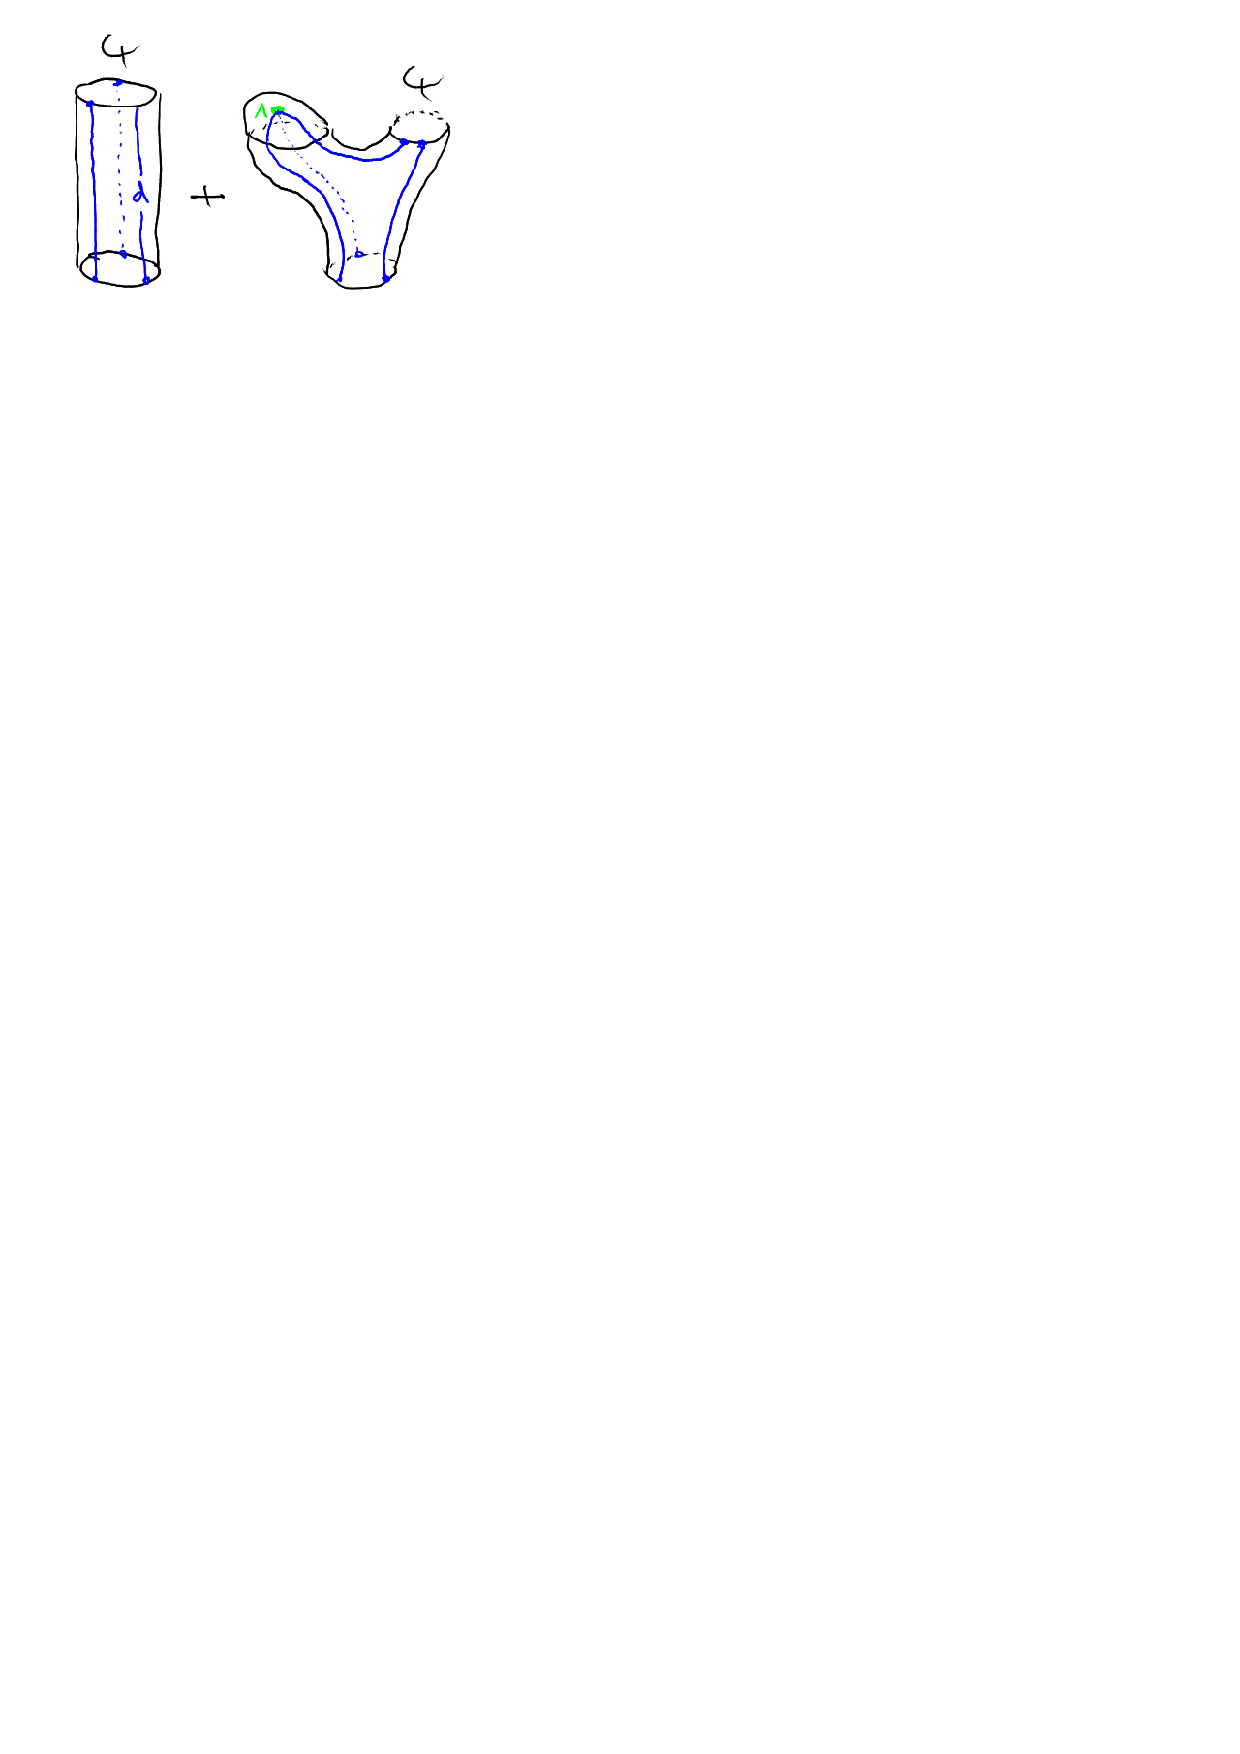
\includegraphics[trim=1cm 24.5cm 12.6cm .4cm]{\GraphicsFolder/diff.pdf}
\end{center}
The term $\OPQ_{210}(S_{\mathrm{int}},\cdot)$ $\OPQ_{110}$ adds one possible $\wedge$-interaction.

There is newly an interaction vertex $\wedge$ and also $\Dd$. If $\OPQ_{210}$ and $\OPQ_{120}$ were well-defined on $\DBCyc\DR$, then the $\dIBL$-algebra 
$$ \Bigl(\DBCyc\DR,\OPQ_{110}^\MC\coloneqq \OPQ_{110} + \OPQ_{210}(S_{\mathrm{int}},\cdot),\OPQ_{210},\OPQ_{120}\cdot\Bigr)$$
would be the $\IBLInfty$-chain model of string topology. 

%They are all define $\dIBL$-structures on $\DR$ then 
%$\Model \coloneqq \CycC(\DR)$ with the $\dIBL$-structure $(\OPQ_{110} + \OPQ_{210}(S_{\text{free}},\cdot), \OPQ_{210}, \OPQ_{120})$ would be the correct $\IBLInfty$-chain model for string topology.  
%Making from operations $V^{\otimes k} \rightarrow V$ is called cyclization and we normaly non-degenerate pairing for that.

As in quantum field theory, we are going to ``formally'' integrate out redundant degrees of freedom in our ill-defined theory and obtain a finite theory on $\DBCyc\HDR$, which is ``formally'' homotopy equivalent to the original one. We pick a Riemannian metric and consider the Hodge decomposition $\DR = \Harm \oplus \Im\Dd \oplus \Im\CoDd$, where $\Harm \simeq \HDR$ are the harmonic forms $\Dd \omega = \CoDd \omega = 0$. For Chern-Simons fields $\omega\in \DR$, one thinks of $\Dd \omega = 0$ as of the Euler-Lagrange equation and of $\CoDd \omega = 0$ as of the Lorentz gauge. The ``inverse'' of $\Dd$ with $\Im\Dd \rightarrow \Im \CoDd$ is the standard Hodge homotopy $\HtpStd$. Its Schwartz kernel is the standard Hodge propagator $\PrpgStd$. A formula for the effective action $W\in\Fun(\BCyc\HDR)$ was given in \cite{Cieliebak2015}; it is of the form
$$ W = \hbar^{-1}\sum_{l\ge 1, g\ge 0} \PMC_{lg} \hbar^{g}, $$
where $\PMC_{lg} \in \hat{\Ext}_l \DBCyc\HDR$ is computed from $(l+g-1)$-loop Feynman diagrams with interaction $\wedge$ and propagator $\StdPrpg$. The twisted string $\BV$-operator on $\Fun(\BCyc\HDR)$ reads
$$ \BVOp^W_s = \hat{\OPQ}^{\PMC}_{110}  +  \hbar{\OPQ}_{210} + \sum_{l\ge 2, g\ge 0} \hat{\OPQ}^{\PMC}_{1lg} \hbar^{g}, $$
where $\OPQ_{110}^\PMC = \OPQ_{210}(\PMC_{10},\cdot) = \OPQ_{210}\circ_1 \PMC_{10}$ and $\OPQ_{1lg}^\PMC = \OPQ_{210}\circ \PMC_{lg}$. The resulting $\IBLInfty$-structure is, in fact, a quantum $\CoLInfty$-structure $(\OPQ_{1lg}^\PMC)$ with Drinfeld-compatible Lie bracket $\OPQ_{210}$. So, this is the $\IBLInfty$-chain model of equivariant string topology which we are interested in. The $\IBLInfty$-quasi-isomorphism to string topology is $F\circ I^*: C(\StringSpace M) \rightarrow \DBCyc \HDR$, where 
$$ F = \HTP_{110} + \HTP_{210}\circ_1 \MC_{10} + \frac{1}{2!} \HTP_{310}\circ_{1,1}(\MC_{10},\MC_{10}) + \dotsb  $$
is a chain map $(\DBCyc \DR,\OPQ_{110}^\MC) \rightarrow (\DBCyc \HDR,\OPQ_{110}^\PMC)$, where $\HTP_{110} = \iota^*$, $\iota: \HDR\simeq \Harm \xhookrightarrow{} \DR$ and $\HTP_{k10}\circ_{1,\dotsc,1}(\MC_{10},\dotsc,\MC_{10})$ adds contributions of trivalent trees like:
$$\underbrace{\vcenterline{\begin{tikzpicture}[scale=1,
every label/.append style={font=\scriptsize},
point/.style={circle,fill=blue!40, inner sep=2pt},
root/.style={circle,fill=red!40, inner sep=2pt},
leaf/.style={circle,fill=green!40!black, inner sep=2pt}
]
\def\vertdist{.8}
\def\hordist{.6}
\node[root] (R) at (0,0) {};
\node[point, label={[right,yshift=-1mm] $\wedge$}] (RU) at ($(R) + (0,\vertdist)$) {};
\node[point, label={[right] $\wedge$}] (RUL) at ($(RU) + (-2*\hordist,\vertdist)$) {};
\node[point, label={[right] $\wedge$}] (RUR) at ($(RU) + (2*\hordist,\vertdist)$) {};
\node[point, label={[right] $\wedge$}] (RULL) at ($(RUL) + (-1*\hordist,1*\vertdist)$) {};
\coordinate (RULR) at ($(RUL) + (\hordist,\vertdist)$);
\coordinate (RURR) at ($(RUR) + (\hordist,\vertdist)$);
\node[leaf, label={[right] $h_1$}] (RULLL) at ($(RULL) + (-1*\hordist,1*\vertdist)$){};
\node[leaf, label={[right] $h_2$}] (RULLR) at ($(RULL) + (1*\hordist,1*\vertdist)$) {};
\node[leaf, label={[right] $h_3$}] (RULRR) at ($(RULR) + (1*\hordist,1*\vertdist)$) {};
\node[leaf, label={[right] $h_k$}] (RURRR) at ($(RURR) + (1*\hordist,1*\vertdist)$) {};
\node[] (RURRL) at ($(RURR) + (-1*\hordist,1*\vertdist)$) {\ \,\dots};
\node (RURL) at ($(RUR) + (-\hordist,\vertdist)$) {\dots};
\draw (R) edge (RU); 
\draw[thick] (RU) -- (RUL) node[below,midway,shift={(-1.5mm,1mm)}] {$\Htp$}; 
\draw[thick] (RUL) -- (RULL) node[below,midway,shift={(-2mm,2mm)}] {$\Htp$}; 
\draw (RULL) edge (RULLL);
\draw (RULL) edge (RULLR);
\draw (RUL) edge (RULRR);
\draw[thick] (RU) -- (RUR) node[below,midway,shift={(2mm,2mm)}] {$\Htp$};
\draw[thick] (RUR) edge (RURL);
\draw (RUR) edge (RURRR);
\end{tikzpicture}}}_{\begin{multlined} \wedge \circ (\Htp \otimes \Htp)\circ (\wedge \otimes \wedge)\circ (\Htp \otimes \Id \otimes \dotsb  \otimes \Id)\\
 \circ (\wedge \otimes \Id \otimes \dotsb \otimes \Id)(h_1, h_2, h_3, \dots, h_k)
\end{multlined}}$$

Note that in order to evaluate trees, we do not need the Schwartz kernel $\Prpg$ (and hence any pairing). The homotopy $\Htp$ is enough, because the graph is directed and we can distinguish inputs and outputs.

The following is an example of computation of a $1$-loop Feynman graph:
 
\begin{center}
\def\BddMin{.2}
\def\BddMaj{.4}
\def\HorLen{2}
\def\PMCVert{1}
\def\PantsVert{2}
\def\PantsPlunge{.5}
\newcommand{\BddSurf}[6][0]{
% #1 rotation (the optional argument)
% #2 is the center, e.g., C1 or 0:1
% #3 is the major semiaxis
% #4 is the minor semiaxis
% #5 is the style of the upper half
% #6 is the style of the lower half
\draw[#5,rotate=#1] ([shift=(0:{#3} and {#4})]#2) arc (0:180:{#3} and {#4});
\draw[#6,rotate=#1] ([shift=(180:{#3} and {#4})]#2) arc (180:360:{#3} and {#4});
%
}
\begin{tikzpicture}[scale=1.5]
\tikzset{point/.style = {draw, circle, fill=black, minimum size=2pt,inner sep=0pt}}
\coordinate (C1) at (0,0);
\coordinate (CC) at ($(C1) + (\HorLen,0)$);
\coordinate (CV) at ($(C1) + (.5*\HorLen,\PMCVert)$);

\coordinate (C2) at ($(CC) + (.5*\HorLen,-\PantsVert)$);
\coordinate (CP) at ($(CC) + (.5*\HorLen,-\PantsPlunge)$);
\coordinate (C3) at ($(CC) + (\HorLen,0)$);
 
\BddSurf{C1}{\BddMaj}{\BddMin}{dotted}{}
\BddSurf{C2}{\BddMaj}{\BddMin}{dotted}{}
\BddSurf{C3}{\BddMaj}{\BddMin}{}{}
\BddSurf{CC}{\BddMaj}{\BddMin}{dotted}{dotted}

\draw ([shift={(\BddMaj,0)}]C1) to[out=90,in=180] ([shift={(0,-\BddMaj)}]CV);
\draw ([shift={(0,-\BddMaj)}]CV) to[out=0,in=90] ([shift={(-\BddMaj,0)}]CC);
\draw ([shift={(-\BddMaj,0)}]CC) to[out=-90,in=90] ([shift={(-\BddMaj,0)}]C2);
\draw ([shift={(\BddMaj,0)}]C2) to[out=90,in=-90] ([shift={(\BddMaj,0)}]C3);
% Lower countour

\draw ([shift={(-\BddMaj,0)}]C1) to[out=90,in=180] ([shift={(0,\BddMaj)}]CV);
\draw ([shift={(0,\BddMaj)}]CV) to[out=0,in=90] ([shift={(\BddMaj,0)}]CC);
\draw ([shift={(\BddMaj,0)}]CC) to[out=-90,in=180] (CP);
\draw (CP) to[out=0,in=-90] ([shift={(-\BddMaj,0)}]C3);
% Upper contour


\BddSurf[90]{CV}{\BddMaj}{\BddMin}{dashed,thick}{thick}
% The joint

\draw[thick] ([shift=(45:{\BddMin} and {\BddMaj})]CV) to[out=0,in=95] ([shift=(-40:{\BddMaj} and {\BddMin})]CC) to[out=-85,in=180] ([shift={(0,.-.25*\PantsPlunge)}]CP) to[out=0,in=-90] ([shift=(-140:{\BddMaj} and {\BddMin})]C3);
% The identity line


%START: Inputs from C1
\draw ([shift=(-60:{\BddMaj} and {\BddMin})]C1) to[out=90,in=180] ([shift=(-20:{\BddMin} and {\BddMaj})]CV);

\draw ([shift=(-110:{\BddMaj} and {\BddMin})]C1) to[out=90,in=180] ([shift=(20:{\BddMin} and {\BddMaj})]CV);

\draw[dashed] ([shift=(125:{\BddMaj} and {\BddMin})]C1) to[out=80,in=180] ([shift=(145:{\BddMin} and {\BddMaj})]CV);
%END: Inputs from C1

%START: Inputs from C2
\draw ([shift=(245:{\BddMaj} and {\BddMin})]C2) to[out=90,in=-80] ([shift=(240:{\BddMaj} and {\BddMin})]CC) to[out=100,in=0] ([shift=(-50:{\BddMin} and {\BddMaj})]CV);

\draw[dashed] ([shift=(110:{\BddMaj} and {\BddMin})]C2) to[out=90, in=-85] ([shift=(90:{\BddMaj} and {\BddMin})]CC) to[out=95, in=15] ([shift=(190:{\BddMin} and {\BddMaj})]CV);

\draw ([shift=(-60:{\BddMaj} and {\BddMin})]C2) to[out=90, in=-110] ([shift=(-40:{\BddMaj} and {\BddMin})]C3);

\draw[dashed] ([shift=(70:{\BddMaj} and {\BddMin})]C2) to[out=90, in=-90] ([shift=(80:{\BddMaj} and {\BddMin})]C3);
%END: Inputs from C2

\node[point] at ([shift=(-140:{\BddMaj} and {\BddMin})]C3) {};
\node[point] at ([shift=(190:{\BddMin} and {\BddMaj})]CV) {};

\node[point] at ([shift=(45:{\BddMin} and {\BddMaj})]CV) {};
\node[point] at ([shift=(-50:{\BddMin} and {\BddMaj})]CV) {};
\node[point] at([shift=(20:{\BddMin} and {\BddMaj})]CV) {};
\node[point] at ([shift=(-20:{\BddMin} and {\BddMaj})]CV) {};
\node[point] at ([shift=(145:{\BddMin} and {\BddMaj})]CV) {};

\node[label={[yshift=.1cm] $\psi$}] at (C3) {};
%\node[label={[yshift=-.9cm] $\omega_1$}] at (C1) {};
%\node[label={[yshift=-.9cm] $\omega_2$}] at (C2) {};
\node[label={[yshift=-.7cm] $\scriptstyle \mathrm{T}$}] at (CP) {};
\node at ([shift={(0,-\BddMin)}]CV) {};

% External labels at the first boundary component
\node[point,style={fill=white},label={[below,yshift=-.1cm,xshift=.1cm] $\scriptstyle h_{13}$}] at ([shift=(-60:{\BddMaj} and {\BddMin})]C1) {};
\node[point,style={fill=white},label={[below,yshift=-.1cm,xshift=-.1cm] $\scriptstyle h_{12}$}] at ([shift=(-110:{\BddMaj} and {\BddMin})]C1) {};
\node[point,style={fill=white},label={[below,yshift=+.1cm,xshift=-.6cm] $\scriptstyle h_{11}$}] at ([shift=(125:{\BddMaj} and {\BddMin})]C1) {};

% External labels at the second boundary component
\node[point,style={fill=white},label={[below,xshift=-.1cm,yshift=-.1cm] $\scriptstyle h_{22}$}] at ([shift=(245:{\BddMaj} and {\BddMin})]C2) {};
\node[point,style={fill=white},label={[left,xshift=-.4cm] $\scriptstyle h_{21}$}] at ([shift=(110:{\BddMaj} and {\BddMin})]C2) {};
\node[point,style={fill=white},label={[below,xshift=.1cm,yshift=-.1cm] $\scriptstyle h_{23}$}] at ([shift=(-60:{\BddMaj} and {\BddMin})]C2) {};
\node[point,style={fill=white},label={[right,xshift=.4cm] $\scriptstyle h_{24}$}] at ([shift=(70:{\BddMaj} and {\BddMin})]C2) {};


% Internal labels of vertices
\node[label={[above,yshift=-.01cm] $\scriptstyle x_1$}] at ([shift=(145:{\BddMin} and {\BddMaj})]CV) {};
\node[label={[above,yshift=-.05cm,xshift=.1cm] $\scriptstyle x_2$}] at ([shift=(45:{\BddMin} and {\BddMaj})]CV) {};
\node[label={[right,xshift=-.07cm,yshift=-.18cm] $\scriptstyle x_3$}] at ([shift=(20:{\BddMin} and {\BddMaj})]CV) {};
\node[label={[right,yshift=-.2cm,xshift=-.1cm] $\scriptstyle x_4$}] at ([shift=(-20:{\BddMin} and {\BddMaj})]CV) {};
\node[label={[below,yshift=-.22cm] $\scriptstyle x_5$}] at ([shift=(-50:{\BddMin} and {\BddMaj})]CV) {};
\node[label={[left,yshift=-.2cm,xshift=.1cm] $\scriptstyle x_6$}] at ([shift=(190:{\BddMin} and {\BddMaj})]CV) {};
\node[font=\footnotesize] (ZZ) at ([shift={(0,-5ex)}]CV) {$\Prpg$};
\end{tikzpicture}
$$\begin{aligned}
&\sum_{a,b}\sum_{c=1}^4 \pm  \mathrm{T}^{ab} \psi(e_a  h_{2,c+2}  h_{2,c+3})  \Bigl(\int_{x_1 x_2 x_3 x_4 x_5 x_6} \Prpg(x_1,x_2)\Prpg(x_2,x_3)\Prpg(x_3,x_4)\\
&\Prpg(x_4,x_5)\Prpg(x_5,x_6)\Prpg(x_6,x_1)\bigl( h_{11}(x_1) h_{12}(x_3)
h_{13}(x_4)\bigr)\bigl(e_b(x_2)  h_{2,c}(x_6)  h_{2,c+1}(x_5)\bigr)\Bigr)
\end{aligned}
$$
\end{center}


Finally, note that from the theory of Koszul operads it is well-known that $\IBL$ is a Koszul dual to $\Frob$ (the coproduct is obtained from the product by dualization). Therefore, it holds $\IBLInfty = \mathcal{C}(\Frob)^*$, which precisely reflects our situation of having a Frobenius structure on $\HDR$ and $\IBLInfty$-structure on $\mathcal{C}\HDR^*$.

\section{Other relevant work}

In \cite{Cohen2001}, there is a homotopy theoretical realization of string topology operations.

In \cite{Cieliebak2007}, they sketch a proof that symplectic field theory of the unit cotangent bundle and equivariant string topology are $\IBLInfty$-quasi isomorphic via a map induced by evaluations at boundaries of the holomorphic curves. The string operations then correspond to codimension $1$ boundary structue of the moduli spaces. In fact, precise formulation of this correspondence was perhaps the main reason for the authors to develop the $\IBLInfty$-chain model of string topology.

An $\IBLInfty$-structure on the singular equivariant chain complex was proposed by \cite{Sullivan2005}. It is constructed using ``diffusion intersection product'' which realizes the intersection on the chain level. In fact, there is much more string operations coming from stacks of Sullivan diagrams than just the bracket and cobracket.

There is a recent construction of chain level non-equivariant string topology on the singular chain complex of $\Loop M$ using fat graphs \cite{Drummond-Cole2015} and the diffusion intersection. It was shown in \cite{Cohen2006} that there is a TQFT of string operations on the non-equivariant homology. The aforementioned reference constructs a chain model for this entire gadget. 

There is an algebraic chain model for non-equivariant string topology in \cite{Chen2012}. An algebraic chain model is also constructed in \cite{Irie2014}. 

K.~Fukaya in his work on Lagrangian submanifolds uses chain level string topology.

%(modulo problems with modding out constant loops and with degree shifts) In fact, there is a richer structure 
%They defined the loop product $\LoopPr$ and the unary operator $\BVOp$ on~$\H(\Loop M)$.  In fact, $\StringOp_2$ and $\StringCoOp_2$ descend from $\LoopPr$ and $\LoopCoPr$, respectively, using the maps $\Mark$, $\Erase$ maps. The following phenomenons occur for a general $n$ and families of loops:
%\begin{itemize}
% \item Shifted grading --- 
% \item Vanishing of small loops --- 
% \item Not being an ideal --- 
%\end{itemize}
%A perfect reference to start with string topology from the point of view of algebraic topology is \cite{Basu2011}. More details and various advanced topics can be found in \cite{LoopSpaces}.
%The precise statement is then the following
%
%\begin{Proposition}[The Chas-Sullivan $\IBL$-structure in the equivariant string topology]
%
%\end{Proposition}

\section{Summary of results}

\begin{enumerate}[label=\arabic*)]

\item A large part of the work was about setting up a formalism and deducing signs for the definition of the formal-pushforward Maurer-Cartan element, aka Chern-Simons Maurer-Cartan element, and the $\IBLInfty$-chain model. Another large part was about understanding what is happening and discovering and formulating the structure and possible claims.

\item We compute the $\IBLInfty$-chain model for $\Sph{n}$ with $n\neq 2$ by finding an explicit Hodge propagator and computing Feynman integrals. In fact, for $n\ge 3$, all integrals which are relevant for the $\IBLInfty$-theory vanish.
 
A trick from \cite{Mnev2009} is based on modifying an abstract Hodge propagator to obtain special properties implying vanishing of the integrals. The author of this thesis was not aware of this trick and tried to compute integrals with an explicit propagator in spherical coordinates for around 3 years until he rediscovered a part of this trick himself. The interesting thing is that the discovery was made via explicit computations, and it was a coincidence that the constructed Hodge propagator satisfied the special properties.
 
\item Using the trick from \cite{Mnev2009}, we generalize the previous computation to geometrically formal manifolds and show that the Feynman integrals vanish provided that $\HDR^1(M) = 0$. For a general manifold, all higher coproducts vanish unless $M$ is a surface or a $3$-manifold with $\HDR^1(M) \neq 0$. In fact, the homotopy type of the $\IBLInfty$-chain model for a manifold with $\HDR^1(M) = 0$ is determined by the tree-level perturbative Chern-Simons theory for a special Hodge propagator.

\item We formulate a conjecture that the $\IBLInfty$-chain model for formal manifolds with $\HDR^1(M) = 0$ is homotopy equivalent to the canonical $\dIBL$-structure. We propose a strategy of proof based on Poincar\'e duality models.
 
\item We prove a proposition that the cyclic homology of a strictly unital $\AInfty$-algebra can be computed from its reduced version. We do it by rewriting the Loday's cyclic homology theory for $\DGA$'s.

\item We relate $\OPQ_{210}$ to Gerstenhaber bracket and cyclization and $\OPQ_{120}$ to the Schwarz's $\BV$-operator and cyclic shuffle product.

\item We extend the $\MV$-formalism to filtered $\MV$-formalism and use it to construct a $\BV$-formulation of the weak $\IBLInfty$-theory. This has the advantage that the exponentials are honest exponentials and honest maps. This will be useful for studying $\BV$-chain complexes.

\item We formulate the composition at $k$-common channels $\circ_k$ using ``heart with veins'' which appears in the iterated bialgebra compatibility condition.

\item We understood the $\BV$-formulation of $\IBLInfty$-theory with actions, effective action and quantum master equation.

\item We find the standard Hodge propagator for $\Sph{2}$ up to constants and prove that it smoothly extends to blow-up.
\end{enumerate}

%\section{Author's commentary}
%
%The idea of Prof.~Cieliebak, first one playing with the formalism and realizing what has been somewhere. The thesis is not about proving theorems but rather about getting acquitented with the field and discovering what might be interesting and how it relates to other fields what is interesting and what has been done somewhere else. Huge part lies on 






\end{document}
